\chapter{Diseño e implementación} % Main chapter title
\label{Chapter3} % Change X to a consecutive number; for referencing this chapter elsewhere, use \ref{ChapterX}
En este capítulo se exponen los componentes del hardware, firmware y software que han sido desarrollados, probados e implementados en el presente proyecto.\\

\definecolor{mygreen}{rgb}{0,0.6,0}
\definecolor{mygray}{rgb}{0.5,0.5,0.5}
\definecolor{mymauve}{rgb}{0.58,0,0.82}

%%%%%%%%%%%%%%%%%%%%%%%%%%%%%%%%%%%%%%%%%%%%%%%%%%%%%%%%%%%%%%%%%%%%%%%%%%%%%
% parámetros para configurar el formato del código en los entornos lstlisting
%%%%%%%%%%%%%%%%%%%%%%%%%%%%%%%%%%%%%%%%%%%%%%%%%%%%%%%%%%%%%%%%%%%%%%%%%%%%%
\lstset{ %
  backgroundcolor=\color{white},   % choose the background color; you must add \usepackage{color} or \usepackage{xcolor}
  basicstyle=\footnotesize,        % the size of the fonts that are used for the code
  breakatwhitespace=false,         % sets if automatic breaks should only happen at whitespace
  breaklines=true,                 % sets automatic line breaking
  captionpos=b,                    % sets the caption-position to bottom
  commentstyle=\color{mygreen},    % comment style
  deletekeywords={...},            % if you want to delete keywords from the given language
  %escapeinside={\%*}{*)},          % if you want to add LaTeX within your code
  %extendedchars=true,              % lets you use non-ASCII characters; for 8-bits encodings only, does not work with UTF-8
  %frame=single,	                % adds a frame around the code
  keepspaces=true,                 % keeps spaces in text, useful for keeping indentation of code (possibly needs columns=flexible)
  keywordstyle=\color{blue},       % keyword style
  language=[ANSI]C,                % the language of the code
  %otherkeywords={*,...},           % if you want to add more keywords to the set
  numbers=left,                    % where to put the line-numbers; possible values are (none, left, right)
  numbersep=5pt,                   % how far the line-numbers are from the code
  numberstyle=\tiny\color{mygray}, % the style that is used for the line-numbers
  rulecolor=\color{black},         % if not set, the frame-color may be changed on line-breaks within not-black text (e.g. comments (green here))
  showspaces=false,                % show spaces everywhere adding particular underscores; it overrides 'showstringspaces'
  showstringspaces=false,          % underline spaces within strings only
  showtabs=false,                  % show tabs within strings adding particular underscores
  stepnumber=1,                    % the step between two line-numbers. If it's 1, each line will be numbered
  stringstyle=\color{mymauve},     % string literal style
  tabsize=2,	                   % sets default tabsize to 2 spaces
  title=\lstname,                  % show the filename of files included with \lstinputlisting; also try caption instead of title
  morecomment=[s]{/*}{*/}
}


%----------------------------------------------------------------------------------------
%	SECTION 1
%----------------------------------------------------------------------------------------
\section{Diseño del hardware por etapas}\label{seccion_hardware}
En esta sección se presentan los circuitos esquemáticos correspondientes a cada etapa individual y su rol en el sistema.
\subsection{Circuito de selección de modo}
En el caso límite donde el nivel del acumulador es bajo y el microcontrolador ordena cambiar su estado a un relay con retención, la energía necesaria para excitar al relay puede generar una caída de tensión significativa en el acumulador. As\'{i}, todo el hardware quedaría totalmente desenergizado sin posibilidad de volver a entrar en operación, a menos que exista una intervención humana.\\
Un caso extremo como el anteriormente mencionado, implica que el hardware debe ser capaz de restablecer su estado de operación normal tras largos períodos de tiempo fuera de servicio, aún después de la salida de servicio por falta de provisión de energía.\\
En la figura \ref{fig:ctoselecciondemodo} se muestra el relay sin retención que se implementó,  presentado en la secci\'{o}n \ref{fig:relay}, como as\'{i} tambi\'{e}n su circuito de mando. Los terminales del transformador de corriente se encuentran conectados por defecto a la etapa de conversión y acumulación de energía (terminales NC1 y NC2). Una vez que la tensión en bornes del acumulador alcanza el valor mínimo para que el conversor DC/DC entre en operación, también lo hace la electrónica sin la necesidad de intervención externa.\\
Cada vez que se desea realizar la medición de corriente, el microcontrolador activa la bobina del relay y desconecta el transformador de corriente del circuito de conversi\'{o}n para conectarlo al circuito de medición de valor RMS.\\
% TODO: \usepackage{graphicx} required
\begin{figure}[h]
	\centering
	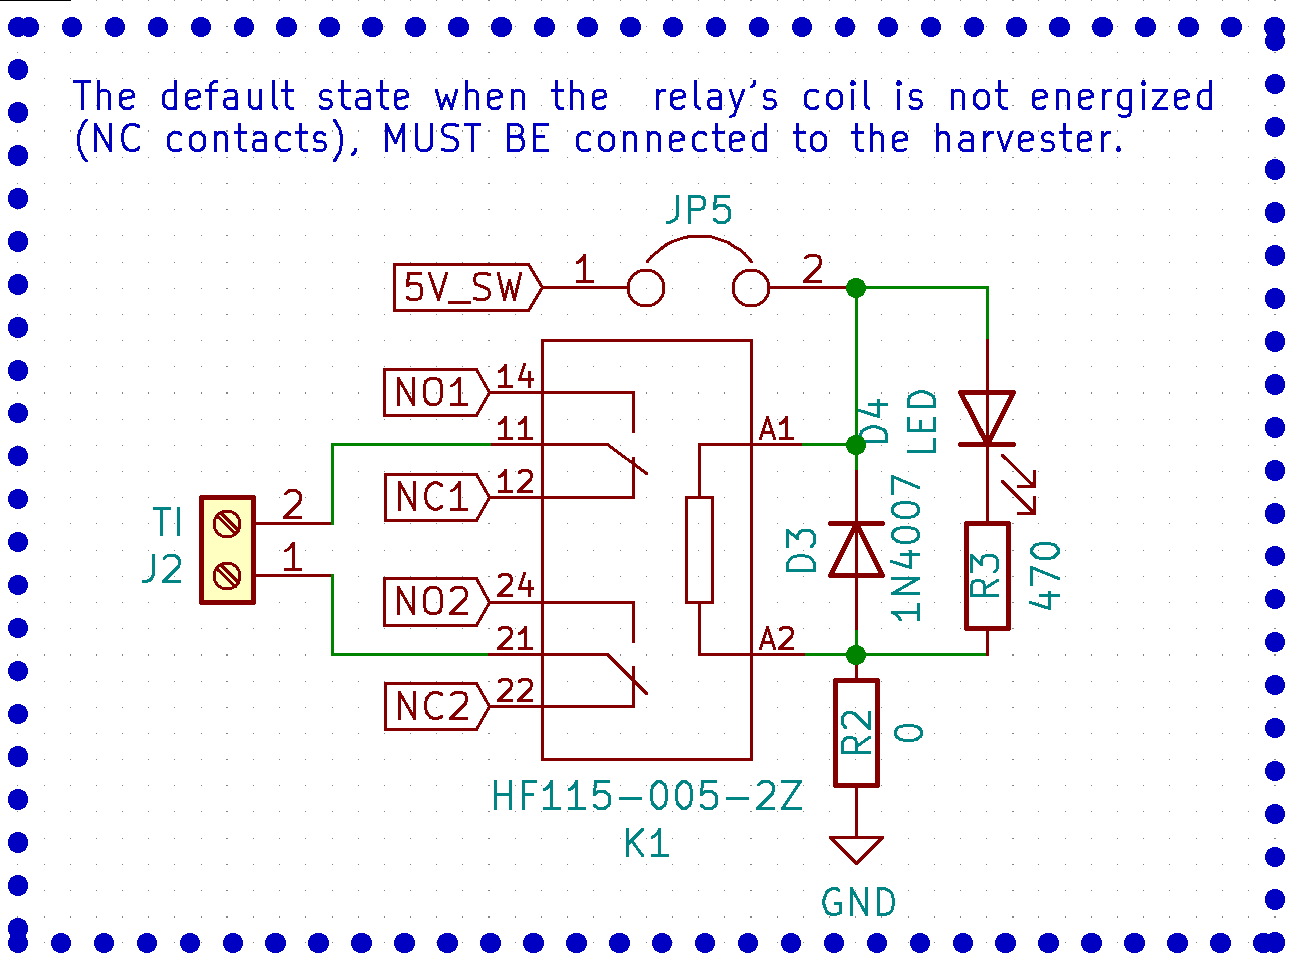
\includegraphics[width=0.8\linewidth]{Figures/cto_seleccion_de_modo}
	\caption{Circuito selector de modo basado en el relay HF115-005-2ZS4.}
	\label{fig:ctoselecciondemodo}
\end{figure}\\

\vspace{10px}
\subsection{Puente rectificador de onda completa}
Para el prototipo desarrollado en este trabajo, se replicó el circuito rectificador de onda completa presentado en la figura \ref{fig:rect_MOSFET}. Con el objeto de reducir el espacio ocupado en el circuito impreso, se optó por utilizar un chip DMHC3025 \citep{dmhc3025}. El encapsulado SOIC-8 presentado en la figura \ref{fig:esquematicointernorctificadormosfet}, alberga un puente H formado por dos transistores MOSFET tipo P y dos tipo N. Las características eléctricas de relevancia para esta aplicación son presentadas en la tabla \ref{tabla_transistores_rectificador}.
% TODO: \usepackage{graphicx} required
\begin{figure}[h]
	\centering
	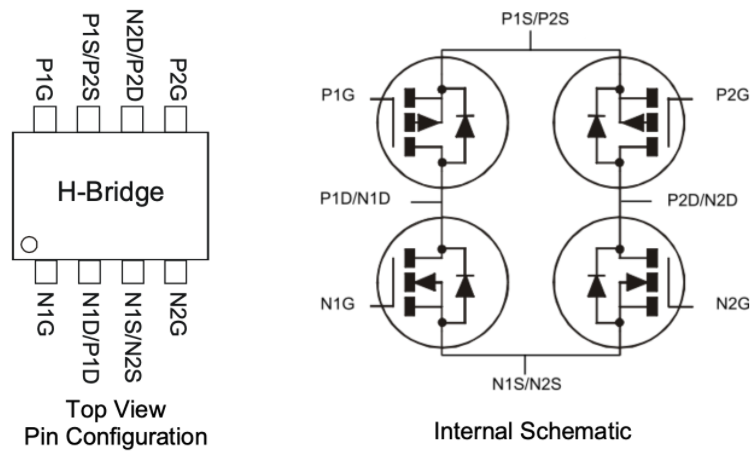
\includegraphics[width=0.7\linewidth]{Figures/esquematico_interno_rctificador_mosfet}
	\caption{Pinout y esquemático interno del DMHC3025 \citep{dmhc3025}.}
	\label{fig:esquematicointernorctificadormosfet}
\end{figure}
\begin{table}[h]
	\centering
	\caption{Características eléctricas de los transistores que forman parte del rectificador de onda completa.}
	\begin{tabular}{cc} 
		\hline
		\textbf{\textbf{Parámetro}} & \begin{tabular}[c]{@{}c@{}}\textbf{}\\\textbf{\textbf{Valor máximo}}\end{tabular}  \\ 
		\hline
		Rds                       & 25 m$\Omega$                                                           \\
		Id                          & 6 A                                                                                \\
		Vdss                     & 30 V                                                                            \\
		\hline
	\end{tabular}\label{tabla_transistores_rectificador}
\end{table}

El circuito final implementado encargado de la rectificación y filtrado de la tensión DC a la salida se presenta en la figura \ref{fig:ctorectificacionfiltrado}. Dos diodos zener D1 y D2 en antiparalelo protegen a los transistores de sobretensión recortando la onda a 27 V para cada semiciclo de la onda senoidal a la entrada.\\
% TODO: \usepackage{graphicx} required
\begin{figure}[h]
	\centering
	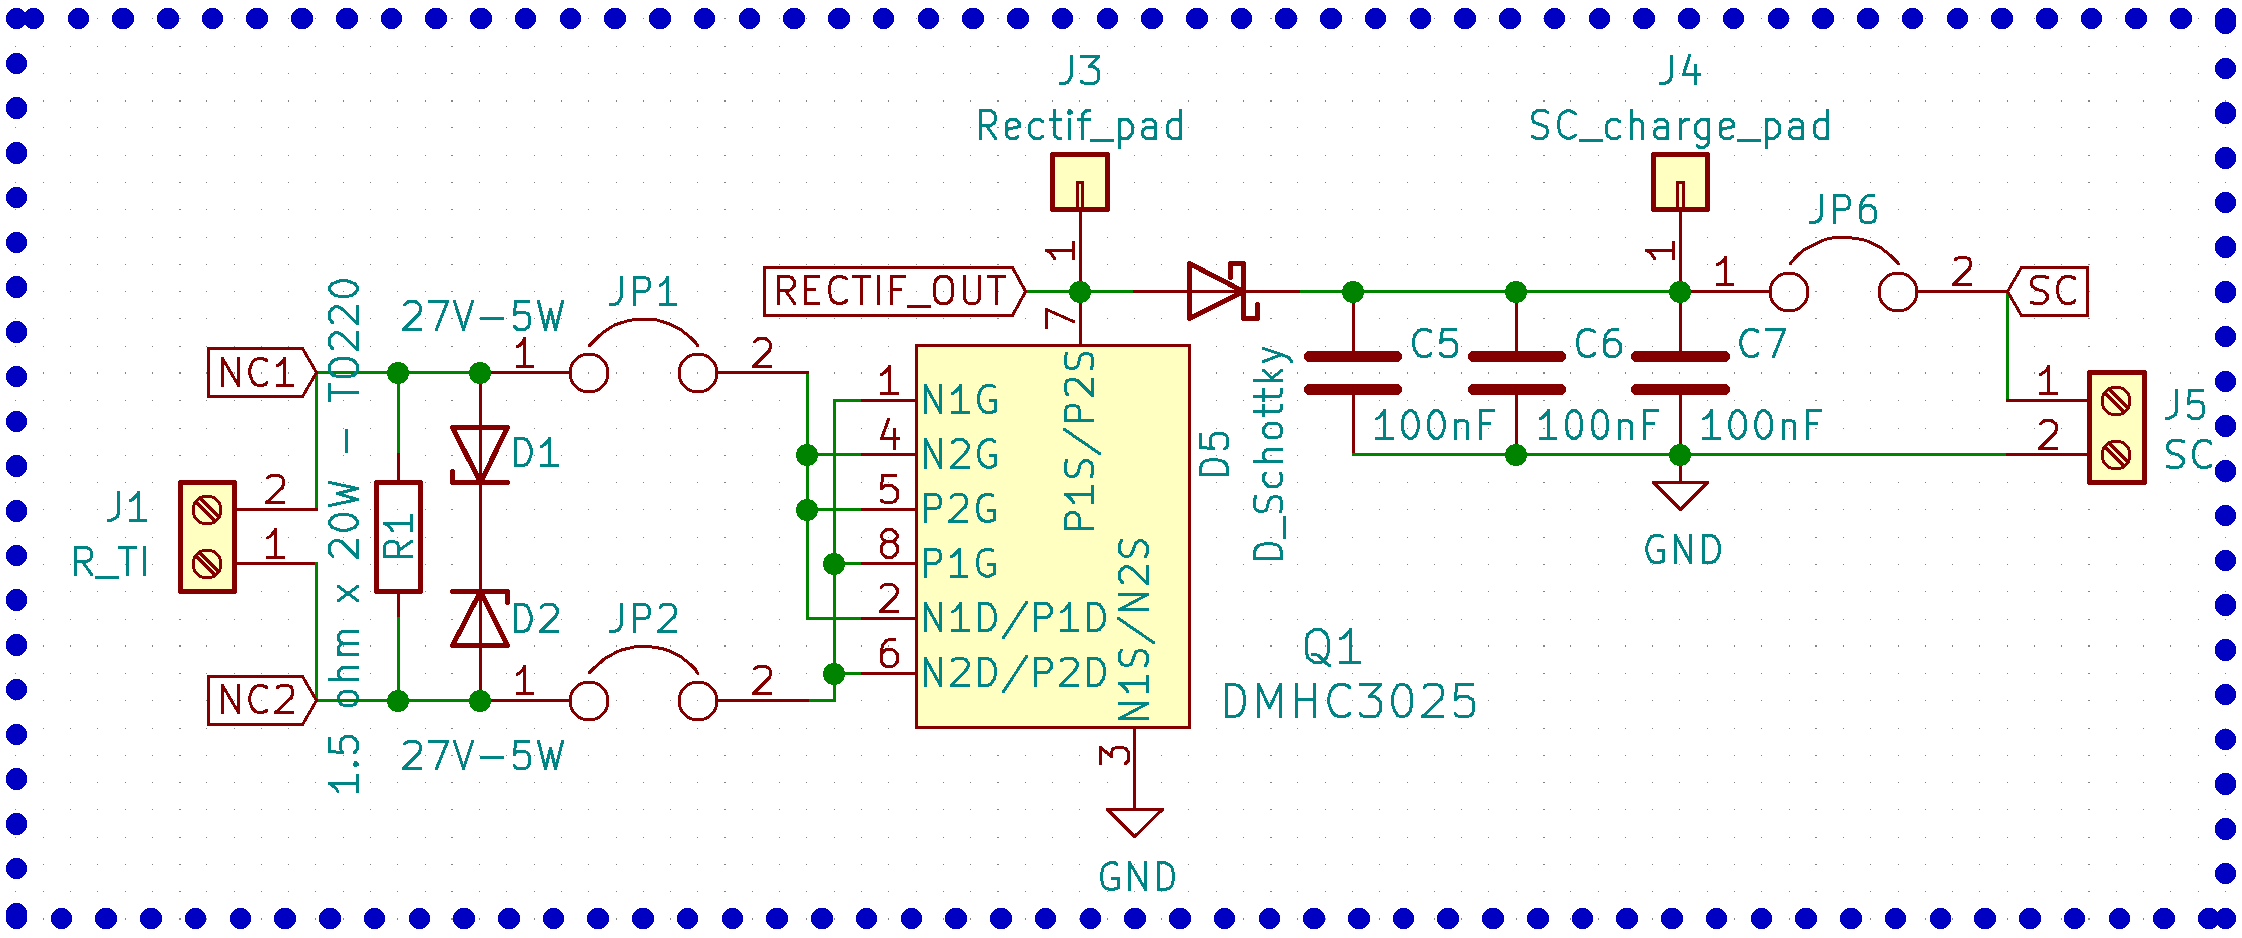
\includegraphics[width=1.0\linewidth]{Figures/cto_rectificacion_filtrado}
	\caption{Etapa de rectificación, filtrado y acumulación implementada.}
	\label{fig:ctorectificacionfiltrado}
\end{figure}\\
A su salida, un conjunto de capacitores cerámicos C5, C6 y C7 filtran ruido de alta frecuencia para luego acumular la energía en el supercapacitor conectado a J5.

\subsection{Acumulador de energía basado en supercapacitores}
A la salida del rectificador de onda completa de la figura \ref{fig:ctorectificacionfiltrado}, se conecta a través de la bornera J5 un banco compuesto por dos supercapacitores de 500 F x 2,7 V en serie, que resulta en una capacitancia equivalente de 250 F x 5,4 V.\\
Los supercapacitores se presentan en la figura \ref{fig:imagensupercap} como un módulo, donde ya se encuentran montados sobre una placa con un circuito adicional de protección. El circuito de protección se encarga de limitar la tensión en sus bornes a 2,5 V y disipar la potencia excedente.\\
% TODO: \usepackage{graphicx} required
\begin{figure}[h]
	\centering
	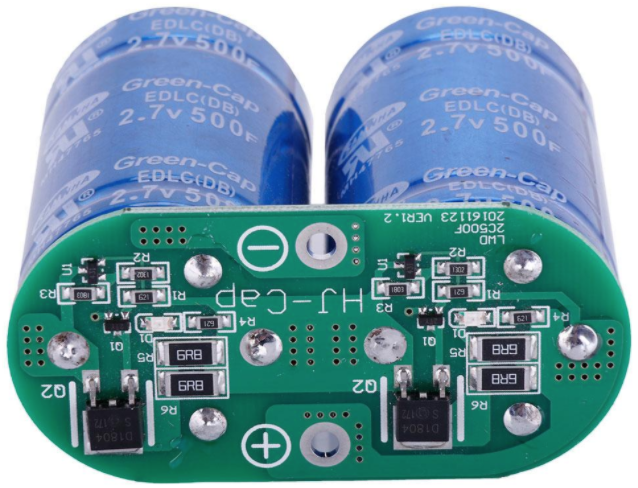
\includegraphics[width=0.5\linewidth]{Figures/imagen_supercap}
	\caption{Banco de supercapacitores de 500 F x 2,7 V utilizado como acumulador.}
	\label{fig:imagensupercap}
\end{figure}\\
Al tratarse de una capacitancia, considerablemente mayor que la de un capacitor habitual, almacena también más energía. El supercapacitor cumple entonces la función de acumular energía para mantener operativa la electrónica en caso de que se interrumpa la conversión de energía.\\
Además de aportar simpleza al esquemático final, el módulo elegido provee un rango de temperatura de operación más amplio que el de una solución que además incluya una batería \citep{PORCARELLI20141671}.\\

 \subsection{Circuito de detección de cortes}
 Una de las funcionalidades relevantes del hardware, es detectar interrupciones en la distribución de energía debido a razones tales como sobrecarga en la línea o desastres naturales.\\
 El circuito detector de cortes propuesto en la figura \ref{fig:ctodetectorcortes} está basado en un comparador TLV3691 de la firma Texas Instruments \citep{tlv3691}. La salida genera una señal de 3,3 V que despierta al microcontrolador por medio de una interrupci\'{o}n por hardware.\\
   % TODO: \usepackage{graphicx} required
 \begin{figure}[h]
 	\centering
 	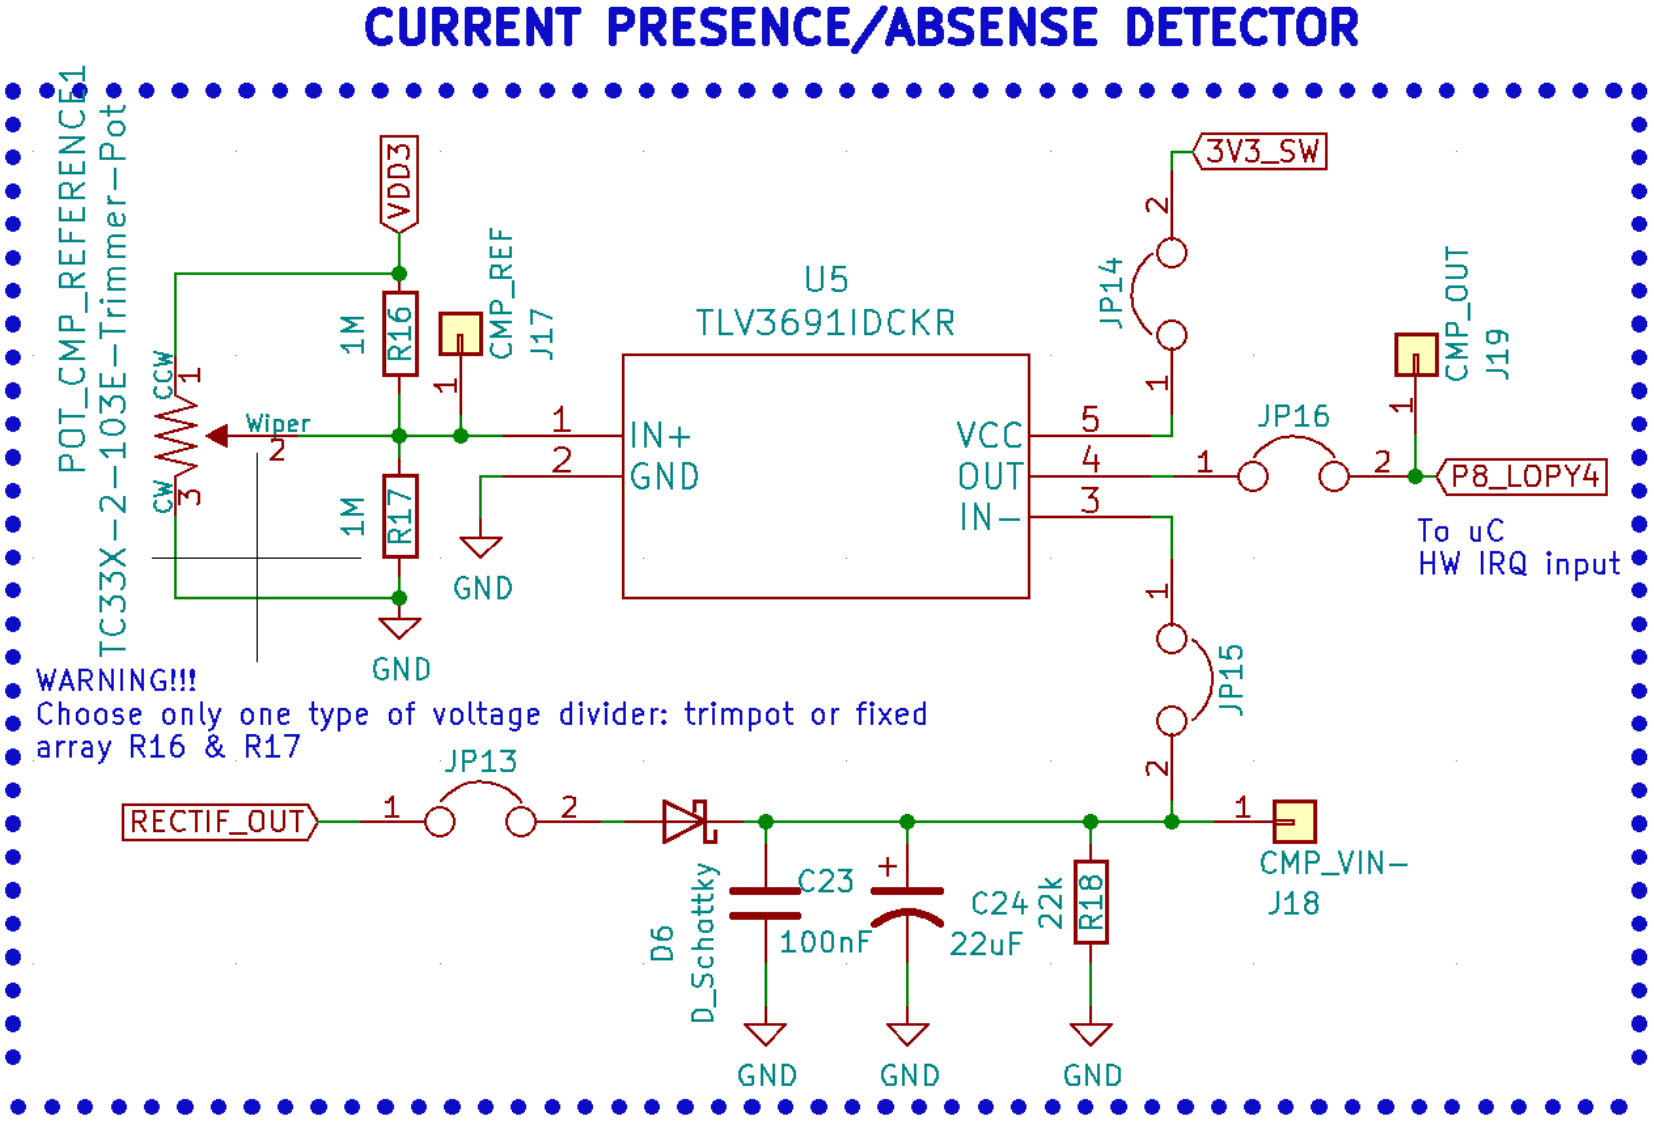
\includegraphics[width=0.9\linewidth]{Figures/cto_detector_cortes}
 	\caption{Circuito detector de cortes basado en el TLV3691 \citep{tlv3691}.}
 	\label{fig:ctodetectorcortes}
 \end{figure}\\
 La salida del puente rectificador se conecta al detector mediante el diodo D6. A continuación los capacitores C23 y C24 filtran el rizado presente en la señal, resultando en una señal DC a la entrada no inversora del comparador.\\
 En el caso de que ocurra un corte en la línea de distribución, la corriente que circula por D6 es nula y los capacitores se descargar\'{a}n a través de R18. Al bajar su tensión por debajo de 1,65 V, la salida se pondrá en alto y la interrupción será atendida por el firmware del microcontrolador.\\
 
 \subsection{Circuito de apagado y encendido mediante load switch}
 Con el objeto de minimizar el consumo en estado ocioso, es necesario desenergizar toda electrónica asociada al hardware que se encuentre en desuso, con excepción del microcontrolador y el circuito detector de la figura \ref{fig:ctodetectorcortes}.\\
 Para interrumpir la alimentación de manera electrónica, se adoptaron dos circuitos independientes basados en un \textit{load switch} FPF2100 de la firma ON Semiconductor \citep{fpf2100}, los cuales se presentan en la figura \ref{fig:ctoloadswitch}.
 % TODO: \usepackage{graphicx} required
 \begin{figure}[h]
 	\centering
 	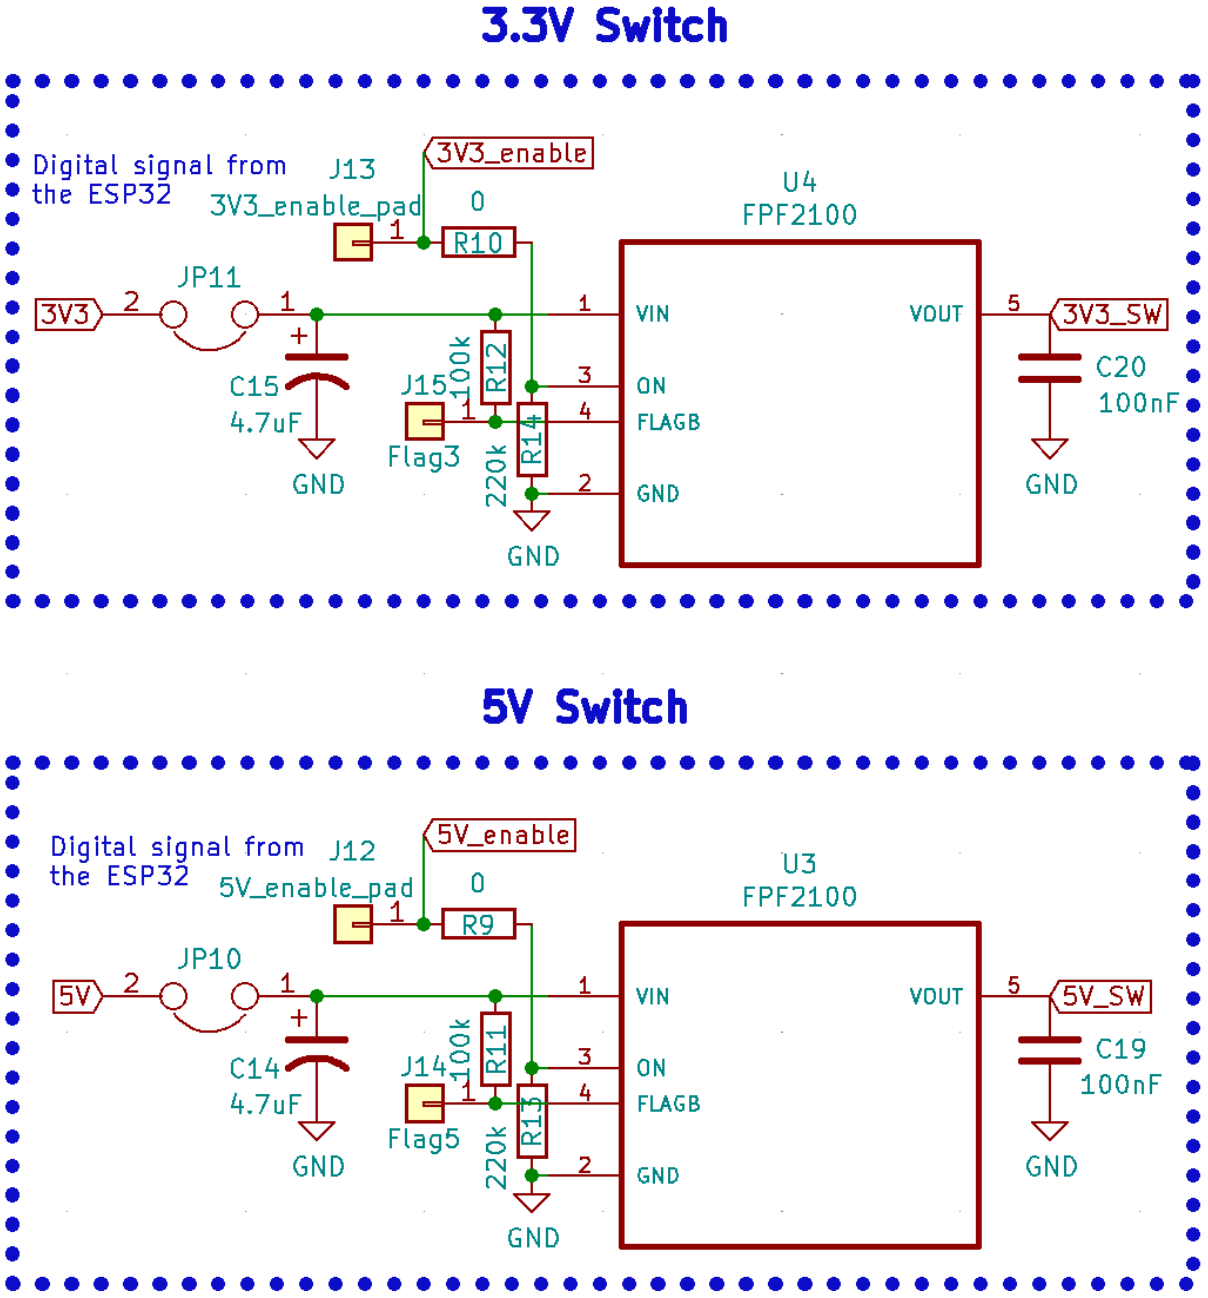
\includegraphics[width=0.8\linewidth]{Figures/cto_load_switch}
 	\caption{Circuito de encendido y apagado de las diferentes etapas de hardware mediante un load switch FPF2100 \citep{fpf2100}.}
 	\label{fig:ctoloadswitch}
 \end{figure}\\
De esta manera las diferentes etapas de 3,3 V y 5 V se energizan únicamente cuando el microcontrolador pone en estado alto el pin ON a la entrada del \textit{load switch}.\\
 
\subsection{Circuito de medición de valor RMS de corriente y acondicionamiento de se�l}\label{circuito_rms}
Para medir corriente mediante un transformador de intensidad, primero es necesario convertir la intensidad en una señal de tensión equivalente y a partir de esta, calcular su valor RMS. Un resistor shunt de 0,1 $\Omega$ con encapsulado TO-220-2 fue adoptado para convertir la corriente del secundario del transformador de intensidad en una señal de tensión apta para realizar su medición RMS.\\
En el mercado existen circuitos integrados dedicados a realizar la medición RMS de señales. Generalmente otorgan una tensión DC a la salida proporcional al valor RMS de la tensión a la entrada.\\
La tabla \ref{tabla_chip_rms} compara el ancho de banda, la tensión pico a pico máxima admitida a sus entradas y la tensión de operación de los posibles candidatos a utilizar en este proyecto.\\
\begin{table}[h]
	\centering
	\caption{Tabla comparativa de chips aptos para medición RMS.}
	\begin{tabular}{cccc} 
		\hline
		Modelo                                & \begin{tabular}[c]{@{}c@{}}Ancho de Banda\\(BW)\end{tabular} & \begin{tabular}[c]{@{}c@{}}Vpp\\(m\'{a}x)\end{tabular} & \begin{tabular}[c]{@{}c@{}}Tensión de\\operación (m\'{a}x)\end{tabular}  \\ 
		\hline
		AD636 \citep{ad636}                                & 1,5 MHz                                                      & 283 mV                                             & 5 V                                                                  \\
		\textcolor[rgb]{0.2,0.2,0.2}{LH0091}\citep{lh0091}  & 2 MHz                                                        & +/- 15 V                                           & 22 V                                                                 \\
		\textcolor[rgb]{0.2,0.2,0.2}{LTC1966}\citep{ltc1966} & 800 kHz                                                      & +/- 1 V                                            & 5,5 V                                                                \\
		\hline
	\end{tabular}\label{tabla_chip_rms}
\end{table}\\
Por disponibilidad del autor al momento del ensayo se eligió el LTC1966 de la firma Linear Technologies \citep{ad636}.\\
El LTC1966 posee dos entradas IN1 e IN2 que se conectan a la señal de tensión generada en bornes del shunt representado por R6 en el esquemático \ref{fig:ctomedidorrms}. A su salida VOUT, otorga una tensión DC proporcional al valor RMS de la señal senoidal inyectada entre IN1 e IN2.\\
Siendo 500 mV el valor de pico de un semiciclo de una onda senoidal en la entrada, el valor eficaz a la salida del circuito integrado est\'{a} dado por la ecuación \ref{eq_vmax}.
\begin{equation}
	\label{eq_vmax}
	Vrms=\frac{Vmax}{\sqrt{2}}=\frac{500}{\sqrt{2}}= 353,55\  mV
\end{equation}
Los capacitores C10 y C12 se encargan de realizar el promedio y filtrar el posible ruido de alta frecuencia.\\
C9 y C11 filtran la tensión de alimentación que energiza al circuito integrado.\\
% TODO: \usepackage{graphicx} required
\begin{figure}[h!]
	\centering
	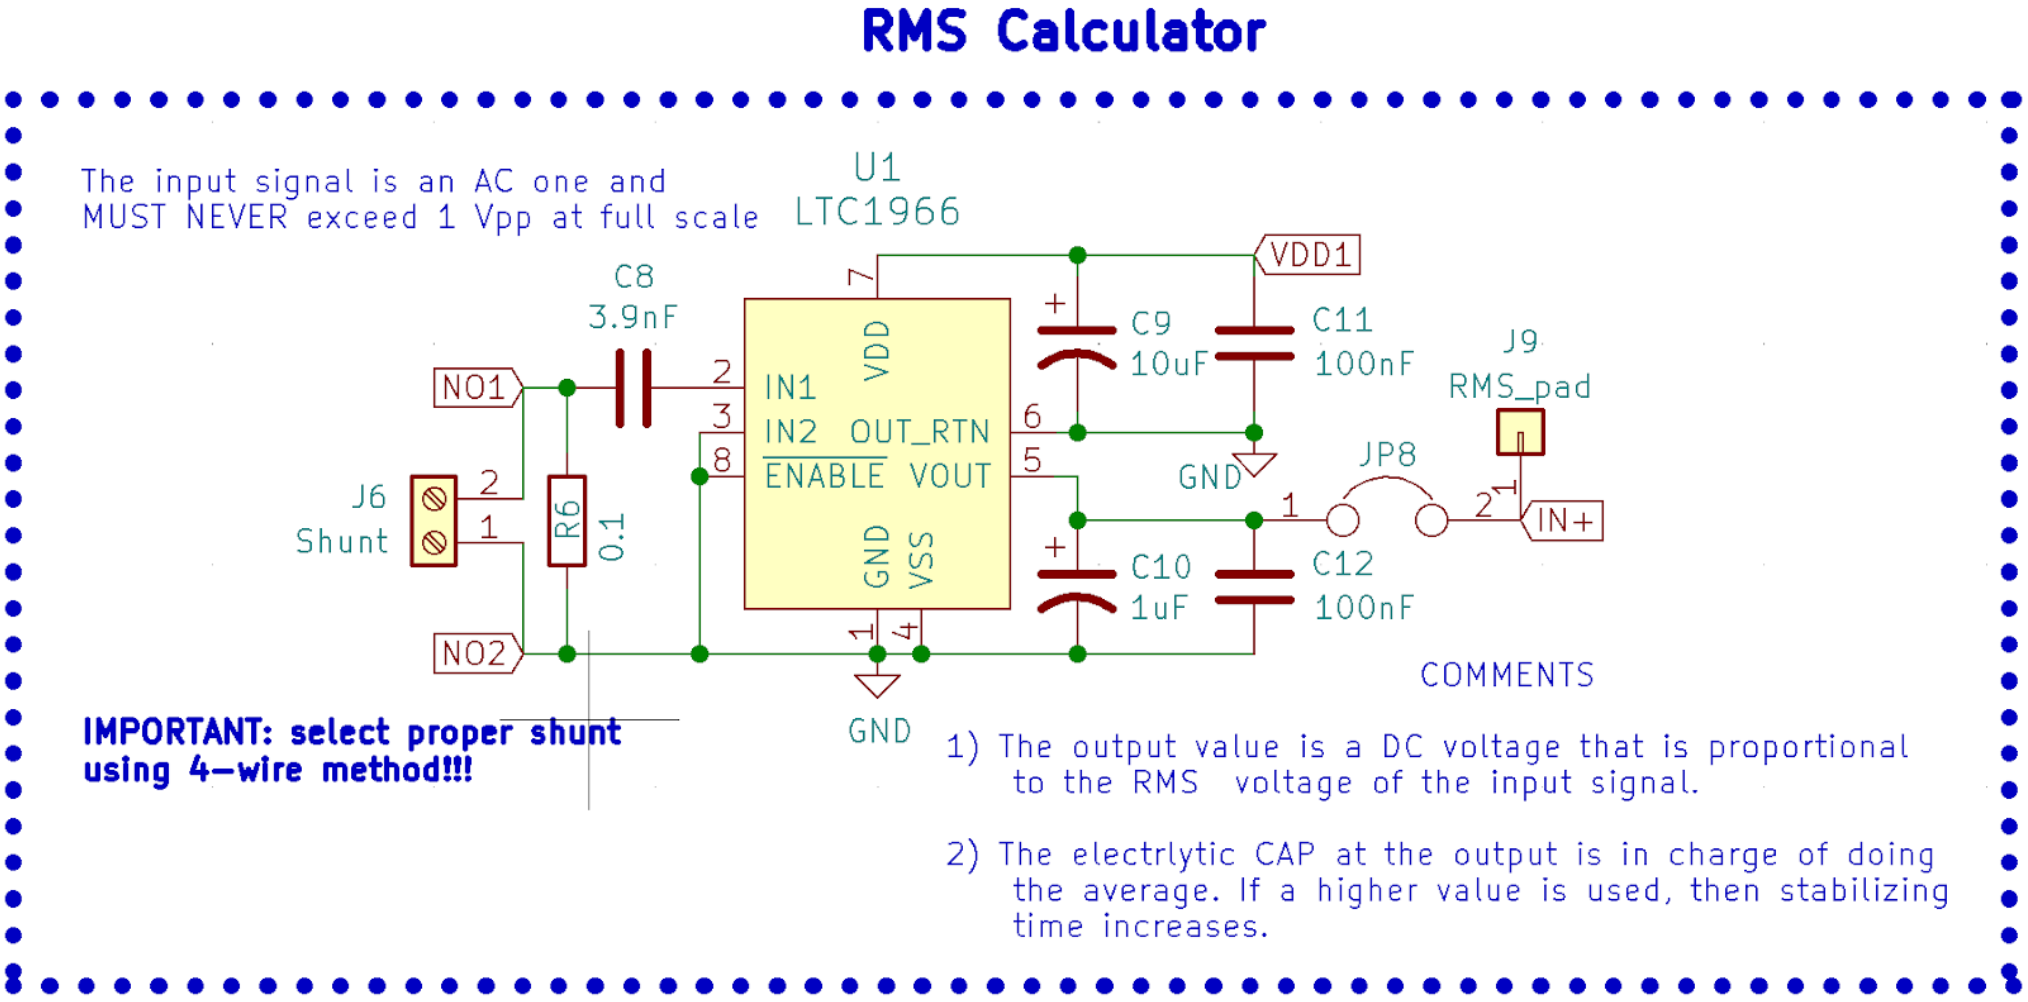
\includegraphics[width=1.0\linewidth]{Figures/cto_medidor_rms}
	\caption{Circuito medidor de valor RMS implementado con el LTC1966.}
	\label{fig:ctomedidorrms}
\end{figure}\\
Dado que las mediciones a realizar se harán en líneas de distribución que operen a 50 Hz o 60 Hz, se ajustó la etapa de filtrado de la señal de entrada. Con una impedancia de entrada de 8 M$\Omega$ entre los pines IN1 e IN2 del LTC1966, el capacitor C8 en serie forma un filtro pasa alto.\\
La frecuencia de corte (fc) adoptada por el autor para este filtro es de 5 Hz y el valor de capacitancia quedó determinado por la ecuación \ref{eq_capacitor_hpf}.
\begin{equation}
	fc = \frac{1}{2.\pi.R.C}\rightarrow\frac{1}{2.\pi.R.fc}\\
\end{equation}
\begin{equation}
	\label{eq_capacitor_hpf}
	C=\frac{1}{2.\pi.{8x10^6}5}=3,978x10^{-9} F
\end{equation}
El valor comercial más próximo adoptado para C8 es 3,9 nF.\\
La señal de salida del LTC1966 es del orden de los mV. Para poder digitalizarla con un conversor analógico-digital es necesario amplificarla de modo que el fondo de escala de la medición tenga como máximo la misma tensión de alimentación que el conversor (3,3 V).\\
El circuito de la figura \ref{fig:ctoopamp}, utiliza un amplificador operacional MP6001U \citep{mcp6001} en configuración amplificador no inversor. La ganancia A del arreglo est\'{a} definida por la ecuación \ref{eq:ganancia}.
\begin{equation}
\label{eq:ganancia}
	A=\frac{R7+Pot1+R8}{R7}
\end{equation}

% TODO: \usepackage{graphicx} required
\begin{figure}[h!]
	\centering
	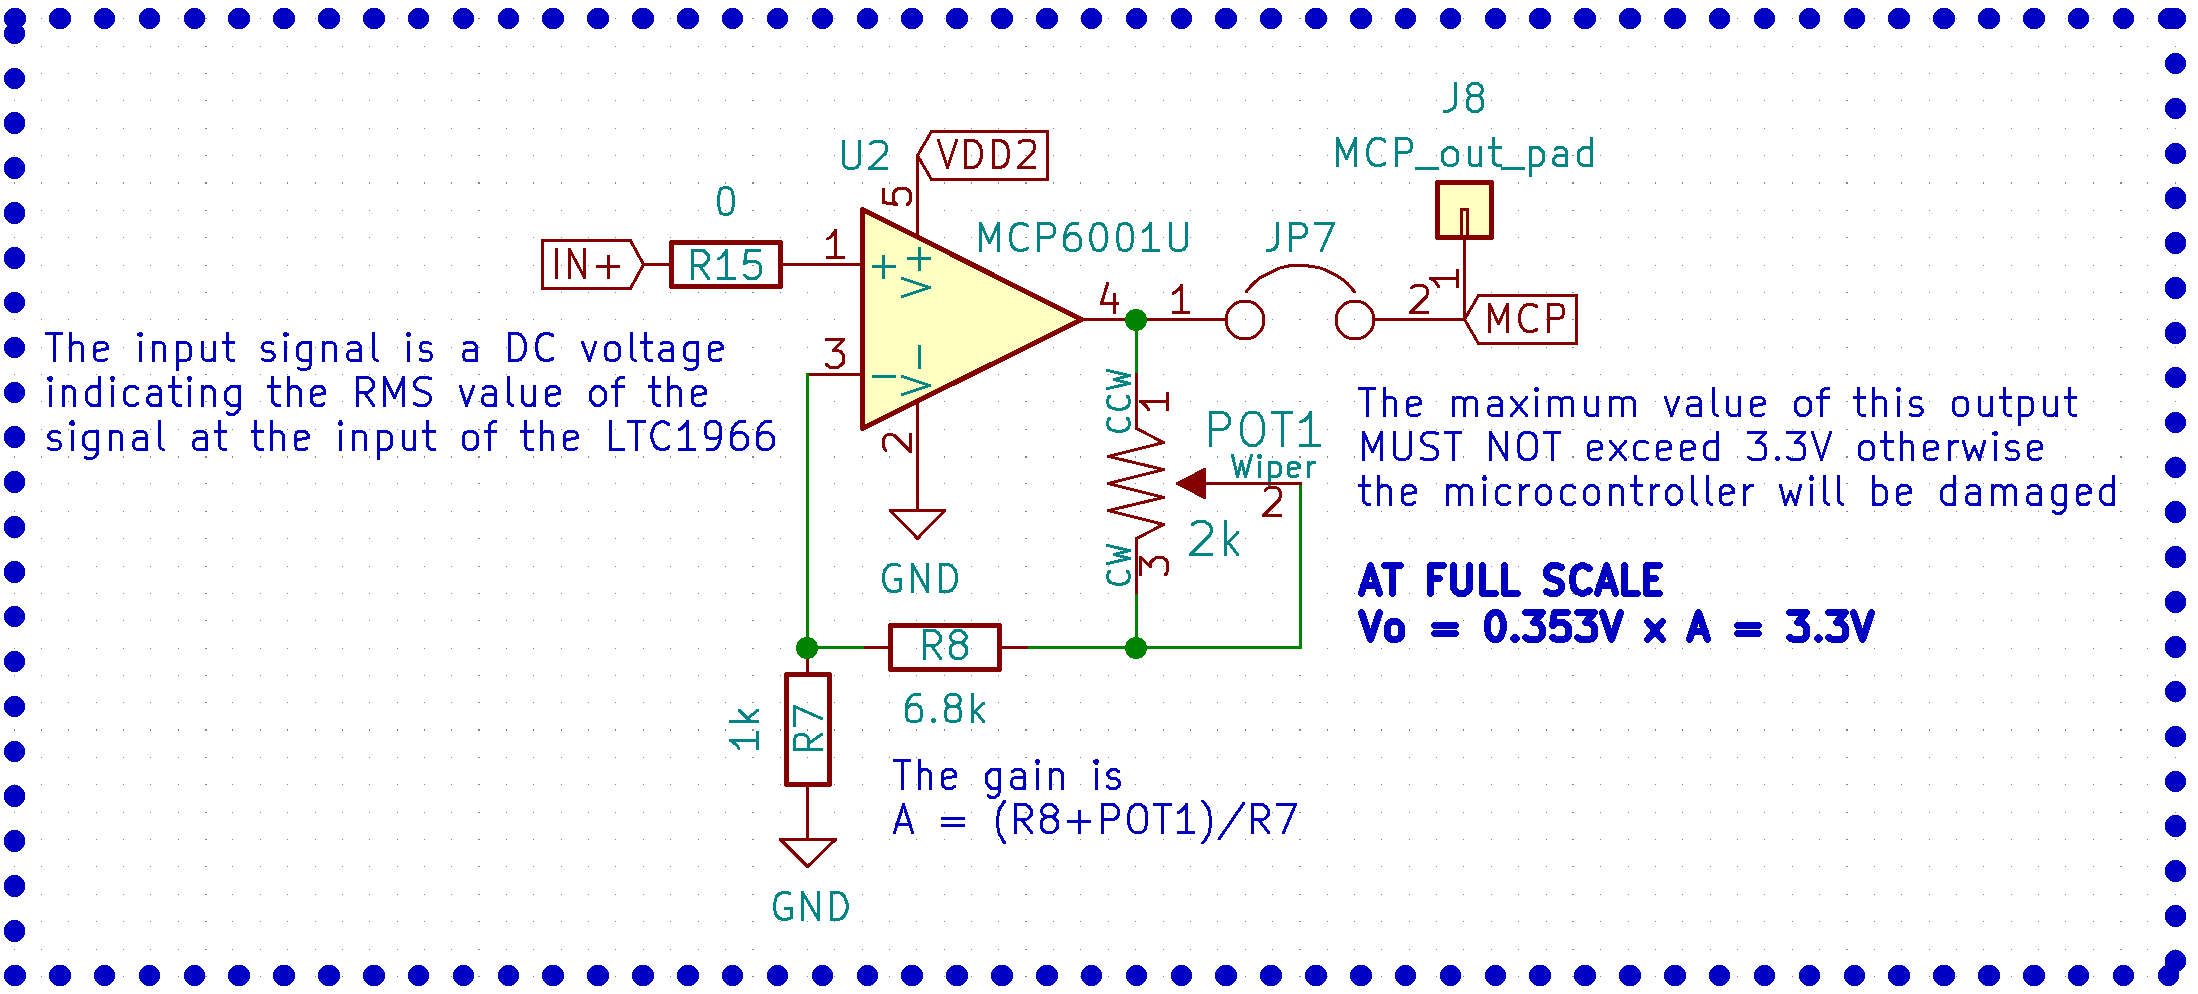
\includegraphics[width=1.0\linewidth]{Figures/cto_op_amp}
	\caption{Circuito amplificador de la señal de salida del LTC1966.}
	\label{fig:ctoopamp}
\end{figure}
El ajuste de la ganancia del amplificador, se realiz\'{o} mediante una tensión de 353,55 mV constante a la entrada IN+ y variando el preset POT1 hasta que la salida alcance 3,3 V. Finalizado el ajuste, la salida se encuentra lista para ser conectada a la entrada del conversor analógico digital.\\

\subsection{Monitoreo de tensión en bornes del acumulador}
La tensión máxima a la que puede llegar el acumulador de la figura \ref{fig:imagensupercap} es 5 V, este valor de tensión es mayor que el máximo admitido por las entradas del conversor analógico-digital (3,3 V). Para obtener una señal de tensión apta y equivalente a la tensión en bornes del acumulador, es necesario atenuar la tensión máxima a medir a un valor de 3,3 V o menos.\\
El divisor resistivo formado por R4 y R5 presentado de la figura \ref{fig:ctodivisorresistivo}, es una solución efectiva para atenuar una señal de tensión DC. De esta manera, un valor de tensión de 5 V en bornes del acumulador, representa como máximo 2,5 V a la entrada del conversor analógico-digital.
% TODO: \usepackage{graphicx} required
\begin{figure}[h!]
	\centering
	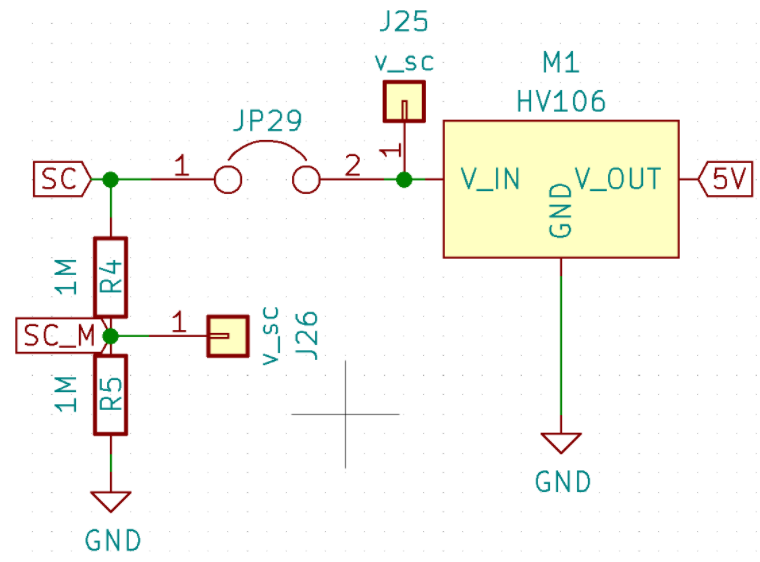
\includegraphics[width=0.6\linewidth]{Figures/cto_divisor_resistivo}
	\caption{Divisor resistivo utilizado para medir la tensión en bornes del supercapacitor.}
	\label{fig:ctodivisorresistivo}
\end{figure}

\subsection{Etapa de conversión analógica digital}
Las señales correspondientes a la tensión en bornes del supercapacitor y valor RMS de corriente son analógicas. Por este motivo, es necesario digitalizar las señales para que luego puedan ser transmitidas por el módulo de comunicaciones.\\
Como solución, en el esquem\'{a}tico de la figura \ref{fig:ctoadc} se adoptó el chip ADS1015 de la firma Texas Instruments \citep{ads1015}. 
El ADS1015 consiste en un conversor analógico digital de 12 bits de resolución, 3,3 V de tensión de alimentación, interfaz de comunicaciones I2C, 4 canales de entrada, tensión de referencia interna y amplificador de ganancia programable.\\
% TODO: \usepackage{graphicx} required
\begin{figure}[h!]
	\centering
	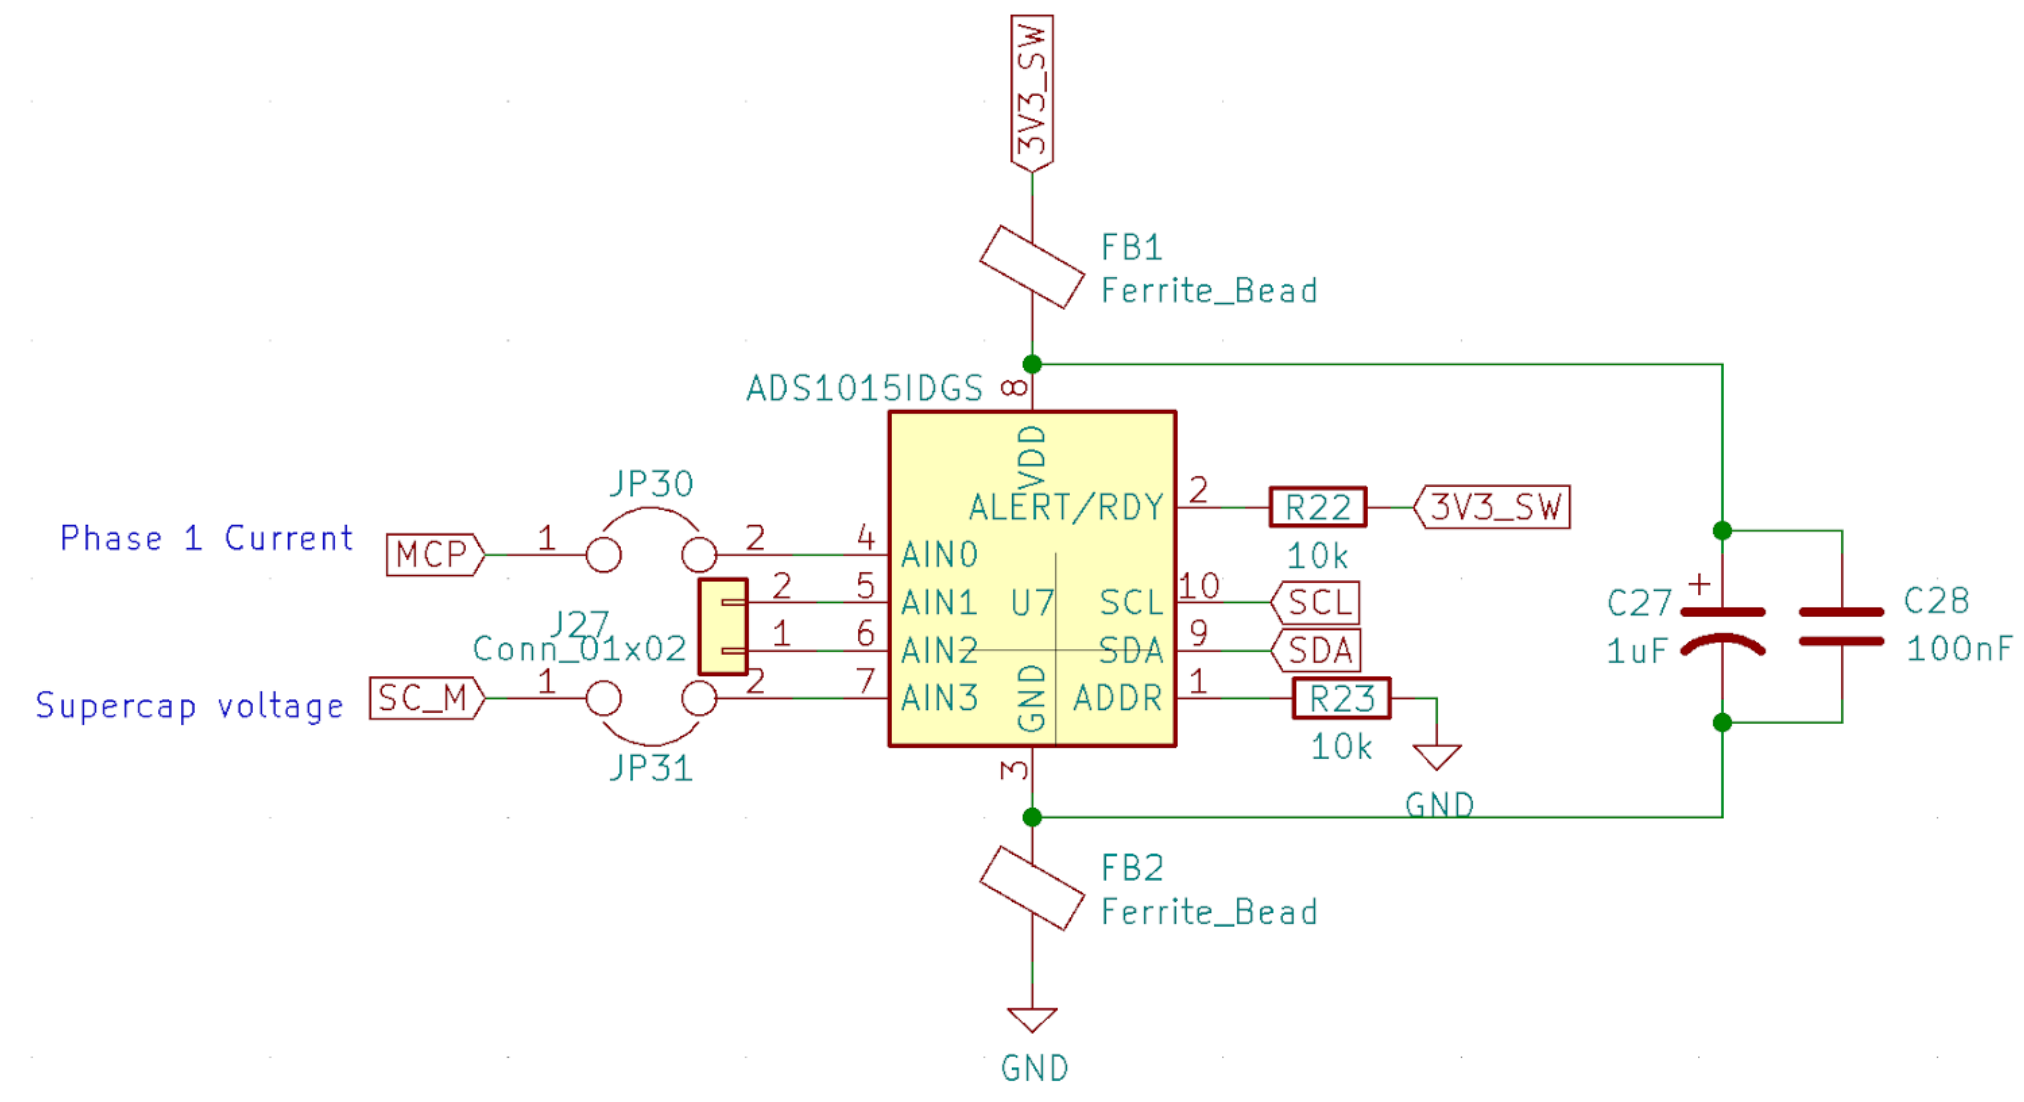
\includegraphics[width=1.0\linewidth]{Figures/cto_adc}
	\caption{Etapa de conversión analógico-digital basada en el ADS1015.}
	\label{fig:ctoadc}
\end{figure}\\
Las señales correspondientes al valor RMS de corriente y tensión en bornes del supercapacitor se conectan a las entradas AIN0 y AIN3 del chip respectivamente. Las restantes entradas AIN1 y AIN2, se conectaron a una tira de pines para agregar de manera opcional otros 2 módulos de medición de corriente.\\


\section{Firmware implementado}
\label{seccion_firmware}
\subsection{Lógica de negocios y patrón arquitectónico adoptado}
Cada hardware tomará una medición y la transmitirá de manera periódica. Al momento de su comisionamiento, el hardware se encontrará en modo conversión y acumulación por defecto.\\
Para lograr la lógica de negocios se adoptó el patrón arquitectónico de la figura \ref{fig:patronpowersaveloop}, resultante de una combinación entre un sistema reactivo y un bucle de ahorro de energía.\\
Al entrar en operación, el microcontrolador verificará que la tensión en bornes del supercapacitor sea mayor a un umbral de 2,5 V antes de enviar su primer reporte de estado. Seguidamente, entrará en modo ahorro de energía o \textit{deep sleep} durante un lapso de tiempo determinado.\\
Si durante el modo \textit{deep sleep} ocurre un corte en el suministro de energía, la señal generada por el circuito de la figura \ref{fig:ctodetectorcortes} hará que el sistema, prematuramente, realice una medición, transmita y nuevamente vuelva a modo ahorro de energía.\\
% TODO: \usepackage{graphicx} required
\begin{figure}[h!]
	\centering
	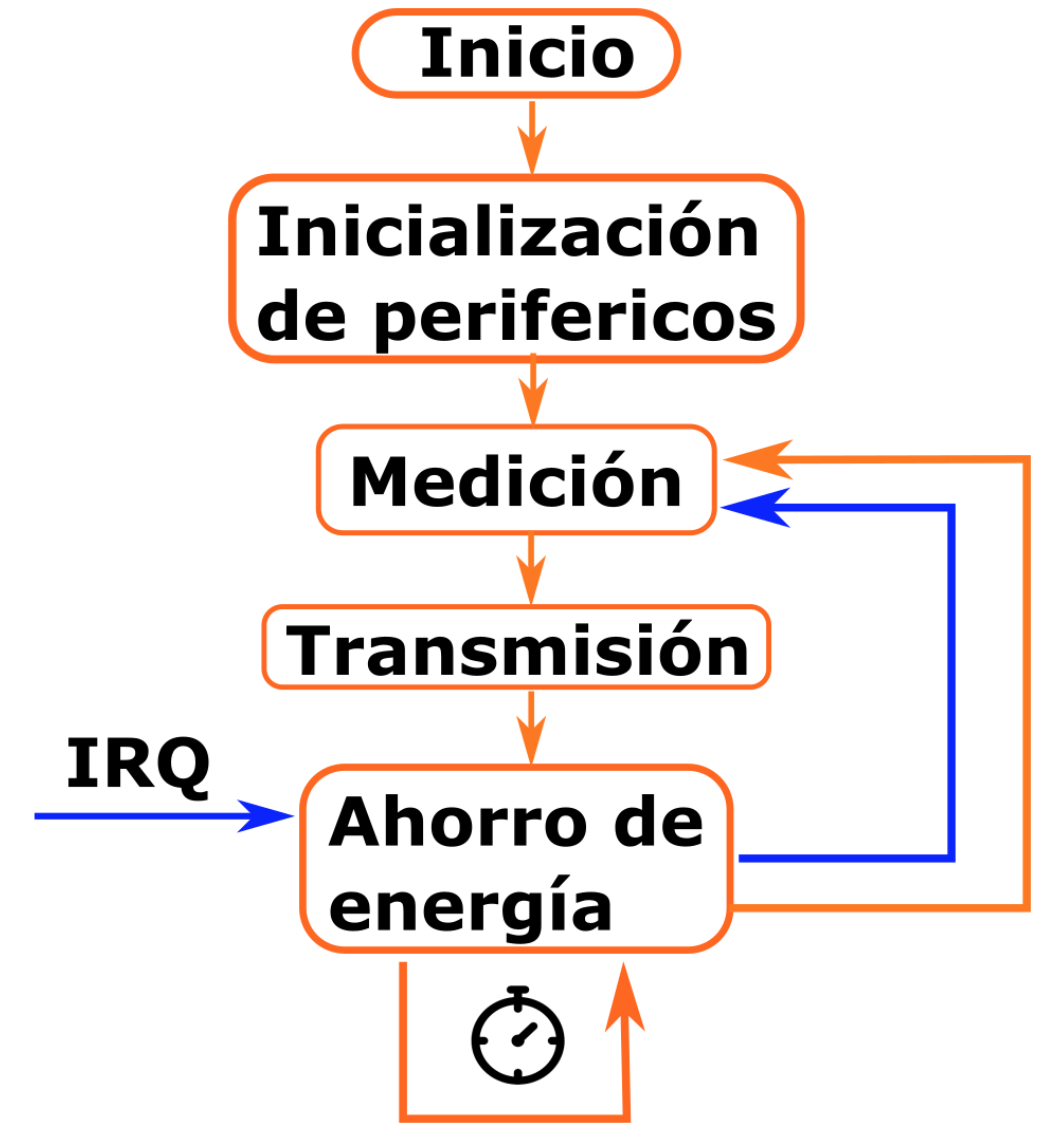
\includegraphics[width=0.7\linewidth]{Figures/patron_power_save_loop}
	\caption{Arquitectura adoptada para la implementación de la lógica de negocios del firmware.}
	\label{fig:patronpowersaveloop}
\end{figure}

\subsection{Inicialización de periféricos}
Esta es la primera tarea que se ejecutará cada vez que ocurre un reset en el microcontrolador.
La tabla \ref{tabla_pines} presenta la función asignada de cada pin físico de la placa de desarrollo LoPy 4, dirección y periférico interno del microcontrolador asociado.\\
\begin{table}[h!]
	\centering
	\caption{Pines de la placa LoPy4 utilizados y los periféricos del ESP32 asociados.}
	\begin{tabular}{ccccc} 
		\hline
		\begin{tabular}[c]{@{}c@{}}Pin\\(LoPy4)\end{tabular} & \begin{tabular}[c]{@{}c@{}}Puerto\\(ESP32)\end{tabular} & Dirección                                               & \begin{tabular}[c]{@{}c@{}}Periférico\\asociado\end{tabular} & Comentarios                                                                 \\ 
		\hline
		2                                                    & P0\_RX0                                                 & entrada                                                 & UART0                                                        & 115200 bps                                                                  \\
		3                                                    & P0\_TX0                                                 & salida                                                  & UART0                                                        & 115200 bps                                                                  \\
		10                                                   & P8                                                      & entrada                                                 & GPIO                                                         & \begin{tabular}[c]{@{}c@{}}IRQ por flanco \\ascendente.\end{tabular}         \\
		11                                                   & P9                                                      & \begin{tabular}[c]{@{}c@{}}entrada\\salida\end{tabular} & I2C                                                          & SDA                                                                         \\
		12                                                   & P10                                                     & salida                                                  & I2C                                                          & SCL                                                                         \\
		13                                                   & P11                                                     & salida                                                  & GPIO                                                         & \begin{tabular}[c]{@{}c@{}}Control del \textit{load} \\\textit{switch} de 3,3 V.\end{tabular}  \\
		14                                                   & P12                                                     & salida                                                  & GPIO                                                         & \begin{tabular}[c]{@{}c@{}}Control del \textit{load} \\\textit{switch} de 5 V.\end{tabular}    \\
		\hline
	\end{tabular} 	\label{tabla_pines}
\end{table}

\subsection{Medición}\label{secc:medicion}
Al cumplirse el per\'{i}odo de ahorro de energía u ocurrir una interrupción, esta función del firmware pone en alto los pines 13 y 14 con el fin de activar los \textit{load switch} de 3,3 V y 5 V para configurar el hardware en modo medición.\\
El relay cambia de estado y conecta el transformador de intensidad al shunt de medición. La etapa de medición de valor RMS formada por los circuitos de las figuras \ref{fig:ctomedidorrms} y \ref{fig:ctoopamp}, otorgan a la entrada del conversor una tensión DC filtrada y acondicionada lista para ser digitalizada.\\
La comunicación con el conversor se realiza a través del bus de comunicaciones I2C. Una biblioteca de libre acceso lista para interactuar con el ADS1015 \citep{upython_ads1015}, se utiliza para tomar 10 valores consecutivos de la señal de interés y almacenarlos en un arreglo. Finalmente se calcula su media aritmética.
El mismo método se invoca para digitalizar la tensión correspondiente al supercapacitor otorgada por el circuito de la figura \ref{fig:ctodivisorresistivo}.

\subsection{Compresión de las mediciones y transmisión a través de LoRa}\label{compresion_lecturas}
Con el objeto de optimizar el tiempo de aire requerido para realizar la transmisión de los datos a la red LoRaWAN, se deben comprimir las lecturas como un conjunto consecutivo de 48 bits.\\
La porción de código presentada en \ref{codigo_compresion}, realiza la compresión de las 4 mediciones recibidas como un arreglo mediante corrimiento de 12 bits para finalmente retornar un valor de 48 bits equivalente a la carga útil.\\

\lstset{language=python}
\begin{lstlisting}[label=codigo_compresion,caption=Función encargada de comprimir las 4 lecturas de 12 bits.]
def compress_analog_reading_payload(self, mediciones):
"""
el orden es mediciones = [0x111, 0x222, 0x333, 0xccc]
para hacer una anidacion de todos tengo que ir corriendo de a 12 bits
# 1 tribble = 3 nibbles = 12 bits
"""
payload = 0
NUMBER_OF_PARAMETERS = 4 # 3 Phase RMS CURRENT readings + SUPERCAP VOLTAGE
DEFAULT_ERROR_PAYLOAD = [3333] * NUMBER_OF_PARAMETERS

if isinstance(mediciones, list) and len(mediciones) == NUMBER_OF_PARAMETERS:
	tribble_shifts = len(mediciones) - 1
else:
	print("ERROR: Did not receive the right amount of params to compress.\
	Was expecting {0} but received {1}."\
	.format(NUMBER_OF_PARAMETERS, len(mediciones)))
	print("Returning: ", DEFAULT_ERROR_PAYLOAD)
return DEFAULT_ERROR_PAYLOAD

if all(isinstance(medicion, int) for medicion in mediciones):
	for medicion in mediciones:
		payload = payload | (medicion << (12 * tribble_shifts))
		tribble_shifts -=1
	return payload
else:
	print("ERROR: not all the elements of the list are INT. VERIFY!!!")
	print("Returning: ", DEFAULT_ERROR_PAYLOAD)
	return DEFAULT_ERROR_PAYLOAD
\end{lstlisting}

Finalizado el ensamblado de la carga útil, se transmite a la red LoRaWAN mediante el transceptor embebido en la misma placa.\\
Una biblioteca provista por Pycom se encarga de gestionar la interacción con las capas superiores del protocolo LoRaWAN para autenticarse y acceder a la red.\\

\subsection{Modo ahorro de energía e interrupciones}
Luego de tomar y transmitir mediciones acorde a lo descrito en \ref{secc:medicion} y \ref{compresion_lecturas}, y antes de configurarse en modo ahorro de energía, el firmware habilita la interrupción por flanco ascendente en el pin 10 de la LoPy4 para permitir que un agente externo haga salir al hardware del modo ahorro de energ\'{i}a.\\
El tiempo t1 requerido para tomar y transmitir mediciones es de tan solo algunos segundos. En comparación con el tiempo t2 en el que el microcontrolador permanece en modo ahorro de energía, que suele ser de varios minutos, puede ser casi despreciable.\\ 
En caso de que no exista una interrupción, el microcontrolador permanecerá en modo ahorro de energía durante un per\'{i}odo t2 hasta cumplir un ciclo T y se restablecerá debido al \textit{timeout} generado (figura \ref{fig:ciclodeepsleep}).\\
% TODO: \usepackage{graphicx} required
\begin{figure}[h]
	\centering
	\includegraphics[width=0.9\linewidth]{Figures/ciclodeepsleep}
	\caption{Ciclo de transmisión, ahorro de energía e interrupciones generadas por cortes.}
	\label{fig:ciclodeepsleep}
\end{figure}\\
Si durante el lapso de tiempo t2 ocurre un corte en el suministro de energ\'{i}a el\'{e}ctrica, el circuito de la figura \ref{fig:ctodetectorcortes} genera una señal de restablecimiento del sistema y el ciclo comienza nuevamente midiendo y transmitiendo.\\


\section{Servicios de Backend}
\label{seccion_bes}
En esta sección se presenta la integración entre los servicios de backend, la red \textit{The Things Network} y la estructura de los datos almacenados para el desarrollo de la interfaz gráfica de usuario.\\
\subsection{Integraci\'{o}n de la red LoRaWAN}
\label{seccion_lorawan}
Cuando la red LoRaWAN recibe la carga útil generada por cada nodo, es necesario realizar el camino inverso al descrito en \ref{compresion_lecturas}.\\
\textit{The Things Network} provee una herramienta dedicada llamada \textit{payload format decoder}. Con esta herramienta cada vez que un paquete de un nodo llega, el código \ref{codigo_descompresion} lo procesa y separa cada lectura como clave de un elemento JSON antes de realizar el env\'{i}o a los servicios de backend.\\
\begin{lstlisting}[label=codigo_descompresion,caption=Función encargada de descomprimir las 4 lecturas de 12 bits.]
function Decoder(byte, port) {
	factor_conversion_corriente = 127/1635;
	
	i1 = ((byte[0] << 4) | (byte[1]>>4))*factor_conversion_corriente;
	i2 = (((byte[1] & 0x0F) << 8) | byte[2])*factor_conversion_corriente;
	i3 = (((byte[3] << 4) | (byte[4]>>4)))*factor_conversion_corriente;
	supercapacitor_adc = (byte[4] & 0x0F) << 8 | byte[5];
	
	FACTOR_DIVISOR_RESISTIVO = 2
	supercapacitor = (((supercapacitor_adc<<4) *4.096/32767))*FACTOR_DIVISOR_RESISTIVO;	
	
	var decoded = {};
	
	decoded.corriente_1 = i1;
	decoded.corriente_2 = i2;
	decoded.corriente_3 = i3;
	decoded.super_capacitor = supercapacitor;

	return decoded;  
}   

\end{lstlisting}
Las primeras experiencias de integración con \textit{The Things Network} se realizaron a través de suscripciones a un tópico de MQTT. Sin embargo, \textit{The Things Network} ya no brinda soporte a este servicio, motivo por el cual se cambió a envíos HTTPs utilizando el método POST.\\
En el servidor web, se encuentra un script PHP (ver anexo \ref{Appendix_PHP_code}) que atiende las consultas que llegan desde \textit{The Things Network}. Este mismo script es el encargado de almacenar los datos en la base de datos.\\

\subsection{Base de datos}
Los datos recibidos a trav\'{e}s de cada petición POST mencionada en la subsecci\'{o}n \ref{seccion_lorawan}, se almacenan de manera cronológica en una tabla llamada \textit{corrientes\_por\_fase}.\\
Las columnas que componen esta tabla y el tipo de dato que almacenan se presentan en la tabla \ref{tablacorrientesporfase}.\\
\begin{table}[h]
	\centering
	\caption{Tabla de la base de datos utilizada para guardar los datos de los nodos.}
	\begin{tabular}{lllccl} 
		\hline
		\multicolumn{1}{c}{Field} & \multicolumn{1}{c}{Type} & \multicolumn{1}{c}{Null} & Key & Default & \multicolumn{1}{c}{Extra}  \\ 
		\hline
		id                        & int(11)                  & No                       & PRI & NULL    & auto\_increment            \\
		id\_sensor                & varchar(40)              & No                       &     & NULL    &                            \\
		datetime                  & datetime                 & No                       & MUL & NULL    &                            \\
		rssi                      & int(11)                  & Yes                      &     & NULL    &                            \\
		snr                       & decimal(6,3)             & Yes                      &     & NULL    &                            \\
		counter                   & int(11)                  & No                       &     & NULL    &                            \\
		v\_supercap               & float                    & Yes                      &     & NULL    &                            \\
		I\_fase\_1                & float                    & Yes                      &     & NULL    &                            \\
		I\_fase\_2                & float                    & Yes                      &     & NULL    &                            \\
		I\_fase\_3                & float                    & Yes                      &     & NULL    &                            \\
		alerta                    & tinyint(1)               & Yes                      &     & 0       &                            \\
		latitud                   & float                    & Yes                      &     & NULL    &                            \\
		longitud                  & float                    & Yes                      &     & NULL    &                            \\
		\hline
	\end{tabular}\label{tablacorrientesporfase}
\end{table}\\
Es relevante destacar que el origen de los datos almacenados, es una combinación entre las mediciones realizadas por el hadware (\textit{I\_fase\_1, I\_fase\_2, I\_fase\_3, v\_supercap}), información acerca de la señal de RF provista por el \textit{gateway} (\textit{rssi} y \textit{snr}) y metadatos propios de cada nodo (\textit{id\_sensor, latitud, longitud}) provistos por el servidor de aplicaciones de \textit{The Things Network}.\\

\subsection{Interfaz gráfica basada en Grafana}
La integración entre MariaDB y Grafana fue inmediata. Gracias a asistentes dedicados, la conexión con la base de datos se redujo únicamente a configurar la dirección del host, usuario y contraseña.\\
La generación de gráficos de corriente por fase se presenta en la figura \ref{fig:historicofase}. La consulta realizada a la base de datos es de pocas líneas y el formato deseado por usuario se ajusta seg\'{u}n cuantas trazas se deseen presentar.
% TODO: \usepackage{graphicx} required
\begin{figure}[h]
	\centering
	\includegraphics[width=1.0\linewidth]{Figures/historico_fase}
	\caption{Gráfico histórico de corrientes de fase.}
	\label{fig:historicofase}
\end{figure}\\
Como único inconveniente se puede mencionar la dificultad que tiene Grafana de manejar muestras temporales si no se utiliza la misma zona horaria que el sistema operativo. En este proyecto se prefirió guardar la información en la base de datos en formato de tiempo universal (UTC). Así, se contribuye a la escalabilidad y robustez del producto, pudiendo desplegarse independientemente de la zona horaria de la instalación.\\
Para subsanar las diferencias entre la base de datos y Grafana se generaron manualmente las consultas SQL agregando el parámetro zona horaria. En la figura \ref{fig:historicofase}, el valor +10800 equivale a los segundos necesarios para compensar en este caso UTC-3.\\
Finalmente en la figura \ref{fig:worldmappanel}, se creó un panel de Worldmap y la consulta SQL se realizó contra una vista que se encarga de recoger los últimos datos individuales de cada nodo.\\
Mediante una herramienta \textit{hover}, una ventana despliega los últimos datos enviados por cada nodo al colocar el cursor sobre el nodo de interés. Esto permite la lectura rápida de los valores de corriente y tensión en el supercapacitor.\\
\vspace{130px}
% TODO: \usepackage{graphicx} required
\begin{figure}[h]
	\centering
	\includegraphics[width=1.0\linewidth]{Figures/worldmap_panel}
	\caption{Panel de Worldmap presentando la lectura de corriente RMS por fase y la tensión del acumulador.}
	\label{fig:worldmappanel}
\end{figure}\\
